% Build: latexmk -pdf talk.tex
\documentclass[aspectratio=169, 11pt]{beamer}

\usetheme{default}
\usecolortheme{beaver}
\setbeamertemplate{navigation symbols}{}
\setbeamertemplate{footline}[frame number]

\usepackage[T1]{fontenc}
\usepackage{lmodern}
\usepackage{amsmath, amssymb, mathtools, bm}
\usepackage{booktabs}
\usepackage{appendixnumberbeamer}
\usepackage{tikz}
\usetikzlibrary{arrows.meta, positioning}

% Reuse the paper's notation so slides and paper agree:
% \input{../paper/macros}

\title{Talk Title as a Claim}
\subtitle{Venue / Seminar}
\author{Author Name}
\institute{Affiliation}
\date{\today}

\begin{document}

\begin{frame}
  \titlepage
\end{frame}

\begin{frame}{The problem matters because \dots}
  \begin{itemize}
    \item<1-> One concrete motivating fact
    \item<2-> What existing methods miss
    \item<3-> What we do differently
  \end{itemize}
\end{frame}

\begin{frame}{Key idea in one picture}
  \centering
  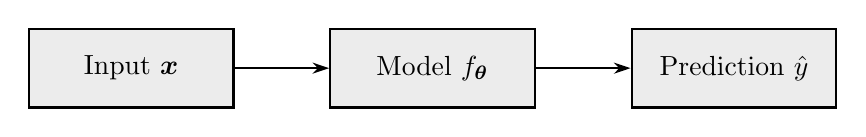
\begin{tikzpicture}[
      block/.style={rectangle, draw, thick, fill=gray!15,
                    minimum width=2.6cm, minimum height=1cm, align=center},
      arrow/.style={-{Stealth[length=6pt, width=4pt]}, thick},
      node distance=1.2cm]
    \node[block] (in) {Input $\bm{x}$};
    \node[block, right=of in] (model) {Model $f_{\bm{\theta}}$};
    \node[block, right=of model] (out) {Prediction $\hat{y}$};
    \draw[arrow] (in) -- (model);
    \draw[arrow] (model) -- (out);
  \end{tikzpicture}
\end{frame}

\begin{frame}{Main result: ours improves accuracy by 3 points}
  \centering
  \begin{tabular}{lc}
    \toprule
    Method & Accuracy (\%) \\
    \midrule
    Baseline & 88.1 \\
    Ours     & \alert{91.3} \\
    \bottomrule
  \end{tabular}
  \note{Mention seeds and variance verbally.}
\end{frame}

\begin{frame}{Take-home message}
  \Large One sentence the audience should remember.
\end{frame}

\appendix
\begin{frame}{Backup: hyperparameters}
  Details for Q\&A.
\end{frame}

\end{document}
